\section{Case Study}
\label{sec:evaluation_openhub}
This section presents a case study of the structural and measurement models using existing software development security data.

We presented the data elements to be collected for our full model in Section ~\ref{sec:model_measurement}, and the data collection guidebook~\cite{morrison2016spefguide} for the measurement model gives instructions on how to collect the data for a software development project. SEM is a large-sample technique, with median sample size in the literature of 200 observations~\cite{kline2015principles}. The need for large quantities of software development security data leads us to examine existing software development security datasets. Further, confirmation of our hypothesized structural and measurement relationships in data we did not generate strengthens the case for the theorized relationships.

At present, no single dataset contains a full set of 200+ projects with data collected using the SP-EF framework. However,  we have identified two datasets that, together, represent most of the  information required for our measurement model:
\begin{itemize}
\item Black Duck Software~\footnote{https://www.blackducksoftware.com/} maintains OpenHub~\footnote{https://www.openhub.net/}, a tracking site for open source software projects. Based on the OpenHub database, Nagappan et al.~\cite{nagappan2013diversity} built and published a dataset of 20,028 projects (OpenHub) to enable assessment of diversity in software engineering research. The OpenHub dataset contains fields related to our Development Risk and Usage Risk constructs, as described below in Section \ref{sec:evaluation_openhub_selection}.
\item The U.S. National Institute of Standards and Technology (NIST) maintains the National Vulnerability Database (NVD) ~\footnote{https://nvd.nist.gov/}, an online database of publicly reported software vulnerabilities, with over 79,000 vulnerabilities dating back to 1988. Vulnerability reporters assign each vulnerability a Common Vulnerability Scoring System (CVSS) score and associated CVSS base metrics, according to the scheme defined in the CVSS guide~\cite{mell2007complete}. 
\end{itemize}

By combining these datasets, we can establish a baseline for assessing the \ModelAbbr.
Our unit of analysis is the software development project. Each Openhub record contains a set of descriptive data about a single project. Each NVD record contains a reported vulnerability for a project. We summarize NVD vulnerability counts for each project. We use the OpenHub projects as our baseline, and include vulnerability counts for OpenHub projects where they have matches in the NVD dataset. We restrict our analysis to those projects which have NVD vulnerability records. The absence of a vulnerability record in the NVD does not mean that a project has no security vulnerabilities, only that vulnerabilities have not been reported. Projects may have no reported vulnerabilities for a variety of reasons, for example, because they are not paid attention to by researchers and attackers, or because they are relatively vulnerability-free. 

We used the R~\footnote{https://www.r-project.org} lavaan package to conduct our SEM analysis, as well as the ggplot2, and semPlot R packages. We now introduce the lavaan syntax, and explain the semantics of each syntax element.

\begin{itemize}
\item Regression relationships between latent variables are specified using the $\sim$  operator (see Table \ref{tab:model_lavaan_syntax}), for example $Outcomes \sim DevelopmentRisk + UsageRisk$ (DevelopmentRisk is also modeled as affecting Outcomes) ("Outcomes are dependent on Development Risk and Usage"). Establishing a parameter estimate for this relationship allows us to test hypotheses about the latent variable relationships, for example the hypothesis that \textbf{H1} Usage Risk is associated with negative Security Outcomes.
 \item Covariance relationships are specified using the $\sim\sim$ operator.
\item Latent variable-measurement variable relationships are specified as follows: $LatentVariable =\sim MeasuredVariable1 + ...$. 
\item Dashed lines indicate estimates established by the researcher, or by the software. We have two examples of modeled fixed parameters in our structural model: We specify the absence of a direct relationship between Usage Risk and Development Risk (syntax: $SoftwareRisk \sim\sim 0*UsageRisk$), as we expect the constructs to be independent of each other. We specify the absence of a direct relationship between Adherence and Outcomes, as we expect Adherence to affect Outcomes through being moderated by overall Development Risk. The remaining dashed lines are estimates fixed by the software, where it has estimated starting values in the course of solving the system of equations expressed by the model.
\end{itemize}

\begin{table*}[!htbp] \centering 
	\caption{Lavaan Syntax} 
	\label{tab:model_lavaan_syntax} 
	\begin{small}
		\begin{tabular}{p{.75cm}p{1.25cm}p{1.5cm}p{3.5cm}p{2.5cm}} 
			&&&&\\[-1.8ex]\hline 
			\hline&&&& \\[-1.8ex] 
			Syntax & Symbol & Name & Description & Example \\ 
			\hline &&&&\\[-1.8ex]  
			$=\sim$	& $\bigcirc \rightarrow \Box$ & is measured by & $=\sim$ specifies how a latent variable (left side) is measured by the constituent variables listed on the right side & $DevelopmentRisk =\sim SLOC + Churn$\\	
			 $\sim$ & $\bigcirc \leftarrow \bigcirc$ & regression & $\sim$ specifies a regression of the dependent variable on the left-hand side to the independent variables on the right hand side of the expression. & Outcomes $\sim$ DevelopmentRisk $+$ UsageRisk  \\	
			 $\sim\sim$ & $\bigcirc \leftrightarrow \bigcirc$ $\Box \leftrightarrow \Box$ & undirected covariance & model a covariance relationship, but leave the direction of influence unspecified. When one side is multiplied by 0, the meaning is that the factors  explicitly do not covary. & $UsageRisk \sim\sim Adherence$  $Adherence \sim\sim 0*Outcomes$\\
			\hline &&&&\\[-1.8ex] 
			\hline &&&&\\[-1.8ex] 
		\end{tabular} 
	\end{small}
\end{table*} 
We now present the complete set of structural model constructs and relationships in the lavaan model syntax: 
 \begin{equation} \label{eq:1}
 \begin{split}
 DevelopmentRisk &=\sim DevelopmentRiskContextFactors\\ 
  UsageRisk &=\sim UsageRiskContextFactors\\
  Outcomes &=\sim OutcomeMeasures\\
  Adherence &=\sim AdherenceMeasures\\
  Outcomes &\sim DevelopmentRisk + UsageRisk\\
   DevelopmentRisk &\sim Adherence\\
   UsageRisk &\sim\sim  Adherence\\
   DevelopmentRisk &\sim\sim 0*UsageRisk\\
   Adherence &\sim\sim 0*Outcomes\\
 \end{split}
 \end{equation}     



%\begin{figure}
% \includegraphics[width=\columnwidth]{modelcaoscto}
%	\caption{Model Constructs and Sub-Constructs}
%	\label{fig:model_constructs_phases}
%\end{figure}


\subsection{Data selection}
\label{sec:evaluation_openhub_selection}
In this section, we describe how we selected each row (observation) and each column(variable) in the source datasets, and how we treated and merged the data. We first present how we interpreted each source dataset field in terms of our structural model concepts. We then present how we merged the datasets into a combined dataset.

The project record contains descriptive data, e.g. project name and version, and security-relevant metrics, e.g. total lines of code (SLOC), and contributor count (Team Size). We now present our mapping of the OpenHub and NVD fields to our \ModelAbbr measurement model metrics.

\subsubsection{Usage Risk}
We map the OpenHub user\_count metric to our Number of Users metric. Number of Users is one of multiple metrics associated with Usage Risk (Table ~\ref{tab:model_spef_metrics}), so this model is a partial account of the factors affecting Usage Risk. 

\subsubsection{Development Risk}
\label{sec:evaluation_openhub_selection_risk}
We model the following Development Risk measurement model metrics based on OpenHub data fields:
\begin{itemize}
    \item SLOC - total\_code\_lines (total\_code\_lines)
    \item Team Size - twelve\_month\_contributor\_count (contributor\_count)
    \item Product Age - difference in months between min\_month and max\_month (product\_age) 
    \item Churn - code\_churn\_12months (code\_churn)
\end{itemize}  

\subsubsection{Adherence}
We do not have direct measures of security practice adherence available in our datasets. We propose an indirect measure, based on inverting Developer Productivity to yield an estimate of development process effort. Developer productivity is sometimes defined (e.g. ~\cite{vasilescu2016the,xuan2014focus,kan2002metrics}) as the ratio of SLOC to unit time per developer. Adherence to software process requirements, including security practices, takes developer time that could be used to write code, suggesting that higher process compliance may be associated with lower SLOC per unit time. We conjecture that inverting the productivity measure yields an indicator of 'developer attention', that will vary, in part, due to the amount of developer time spent on software process activities other than the addition of code. Based on the data available in our dataset, we define this Developer Attention metric as the ratio of developer count over the last 12 months to the code churn over the last 12 months. 

\subsubsection{Outcomes}
We obtain a metric for Outcomes by counting per-project vulnerabilities as of the end of 2012 for each project in the NVD. We treat each unique software name in the NVD records as a distinct project, and sum all vulnerabilities for a project, reflecting our measurement model vulnerability count metric. 

\subsection{Data collection}
For each project, Openhub included SLOC, Language, Contributor Count, Code Churn over the preceding 12 months, Commits over the preceding 12 months, Project Age, and Project Activity. Nagappan et al's~\cite{nagappan2013diversity} inclusion criteria required that each project had at least two committers between June 2011 and June 2012, complete data for all collected fields, and no invalid data (e.g. negative SLOC.)

We included all 20,028 OpenHub projects in the 'Combined' dataset~\footnote{We make our scripts for all described steps available online at www.github/com/pjmorris/Quantifying}. We present summary statistics for the OpenHub dataset in Table \ref{tab:openhub_demog}. We grouped NVD records by project name, and summed vulnerability counts as of the end of 2012 for each project name (in keeping with the time period represented by the OpenHub dataset). We then augmented the Openhub project data with a vulnerability count field, reporting the NVD vulnerability count for the 698 projects that matched by name, and 0 for the remaining projects. We dropped one project which had a total\_code\_lines value of 258 million lines of code, roughly triple the size of Windows as an outlier, yielding a dataset of 697 projects for further analysis.

% stargazer(tr[tr$CVECount>=0,c("total_code_lines.x","twelve_month_contributor_count.x","project_age","code_churn_12months","CVECount","DevChurnAdh12","user_count")])
% Table created by stargazer v.5.2 by Marek Hlavac, Harvard University. E-mail: hlavac at fas.harvard.edu
% Date and time: Mon, May 15, 2017 - 11:46:03
\begin{table}[!htbp] \centering 
  \caption{Combined Project Demographics} 
  \label{tab:openhub_demog} 
\begin{tabular}{@{\extracolsep{5pt}}lrrrrr} 
\\[-1.8ex]\hline \\[-1.8ex] 
Statistic & \multicolumn{1}{c}{N} & \multicolumn{1}{c}{Mean} & \multicolumn{1}{c}{St. Dev.} & \multicolumn{1}{c}{Min} & \multicolumn{1}{c}{Max} \\ 
\hline \\[-1.8ex] 
total\_code\_lines & 697 & 666,297.70 & 2,18,927.00 & 56 & 26,915,903 \\ 
twelve\_month\_contributor\_count & 697 & 34.57 & 90.09 & 2 & 1,167 \\ 
project\_age & 697 & 99.20 & 55.70 & 1.97 & 355.23 \\ 
code\_churn\_12months & 697 & 544,547.20 & 2,195,992.000 & 0 & 25,239,730 \\ 
CVECount & 697 & 11.33 & 45.82 & 1 & 776 \\ 
DevAttention & 697 & 0.04 & 0.69 & 0.00000 & 18.000 \\ 
user\_count & 697 & 260.68 & 901.38 & 0 & 11,150 \\ 
\hline \\[-1.8ex]
\end{tabular} 
\end{table}

\subsection{Estimation}

Combining the structural and measurement models we have defined with the subset of data available in the Combined dataset, we have the model definition, expressed in lavaan syntax: 

\begin{equation}
\begin{split}
	DevelopmentRisk &=\sim total\_code\_lines + twelve\_month\_contributor\_count +\\ 
	& project\_age + code\_churn\_12months\\
 Outcomes &=\sim CVECount \\
 Outcomes &\sim DevelopmentRisk + UsageRisk\\
 Adherence &=\sim DevAttention\\
 DevelopmentRisk &\sim  Adherence\\
 UsageRisk &=\sim user\_count\\
\end{split}
\end{equation}		

\subsection{Model Fit} 

To avoid estimation problems caused by ill-scaled covariance matrices (high ratio between the largest and smallest variances), Kline~\cite{kline2015principles} recommends rescaling variables with low or high variances relative to the other variables in the dataset. We implemented rescaling by applying R's scale function defaults to each variable, subtracting the column mean from each variable, and dividing each variable by its standard deviation.

Standard SEM estimation assumes multivariate normally-distributed variables~\cite{kline2015principles}, pp. 74-78, and normally-distributed joint distributions between variables, however SEM methodologists have develped procedures and estimators for non-normal data. As our data consists primarily of counts, we checked for skewness (ranging from 2.29 for user\_count to 76.48 for total\_code\_lines) and kurtosis (ranging from 12.23 for project\_age to 7993.58 for total\_code\_lines), indicating that we have varying degrees of non-normality in our data. Where data is expected to be non-normal, as with counts, Kline~\cite{kline2015principles}, pp.238-9, recommends  using robust maximum likelihood (RML) to estimate the model, as it does not assume normality, but estimates parameters for each variable's distribution based on the data for each variable. Lavaan implements RML through the MLR estimator. 
 
Applying the described estimation procedure to our transformed data ~\footnote{As a reminder, our scripts are available at ~\url{https://github.com/pjmorris/paper_modeling-sp/blob/master/CombinedCaseStudy.R}}, yielded global fit indicators that were outside the range of standard fit criteria thresholds for CFI, RMSEA and SRMR, as shown in the Combined column of Table \ref{tab:results_fit_combined}. We examine fit refinement in the next section. 

\begin{table*}
	\begin{center}	
		\caption{Global Fit Measures and Results}
			\label{tab:results_fit_combined}
			\begin{tabular}{p{3cm}p{1cm}|p{2cm}p{2cm}}
				\\[-1.8ex]\hline 
				\hline \\[-1.8ex] 
				Fit Measure & Threshold & Combined	& Respecified \\
				Number of observations &  & $697$  & $697$   \\				
				Model chi-square &  & $63.00$ & $71.20$   \\				
				Model d.f. &  & $13$ & $10$   \\		
				Model p-value & $\leq 0.01$ & $0.0$ & $0.0$   \\
				Robust RMSEA & $\leq 0.10$ &  $0.15$ &  $0.10$    \\
				Robust CFI & $> 0.90$ & $0.81$ & $0.94$  \\
				SRMR & $< 0.08$ & $0.11$ & $0.04$  \\
				\hline \\[-1.8ex] 				
			\end{tabular}
	\end{center}
\end{table*}

\subsection{Re-specification}
After reviewing the lavaan modification indice recommendations and what we expect the data to mean, we added three co-variance relationships, as follows:
\begin{itemize}
   \item $total\_code\_lines \sim\sim code\_churn\_12months$. We reason that the relationship is reasonable in light of theory because larger projects tend to have more lines of code available to change.
   \item $twelve\_month\_contributor\_coin \sim\sim code\_churn\_12months$. We reason that the relationship is reasonable in light of theory because larger numbers of contributors are likely to change more code.
   \item $DevAttention \sim\sim 1*DevAttention$. The given expression constrains the variance of DevAttention to 1. As the scaling performed on the data already yields a variance of 1 for DevAttention, this expression simplifies the estimation procedure by preventing it from estimating some other value.
\end{itemize}

The re-specified model had global fit characteristics within the traditional fit criteria thresholds, as shown in the Respecified column of Table \ref{tab:results_fit_combined}. We present the parameter estimates for the Respecified model in the results, and discuss the implications in Section \ref{sec:case_openhub_discussion}.

\subsection{Reporting Results}
\label{sec:case_openhub_results}

We present the global fit results for the Combined and the Respecified models in Table \ref{tab:results_fit_combined}. We report the estimated parameter values, standardized, for the Respecified NVD structural and measurement models in Table \ref{tab:results_openhub}~\footnote{Standardized SEM parameter values are correlations, and can be interpreted as for regression.}. We present the standardized parameter estimates, and the residuals, in the context of the full structural and measurement models in Figure \ref{fig:openhub_model_respecified_estimates}.

\begin{table}
	\begin{center}	
		\caption{OpenHub-NVD Respecified Model Results}
		\label{tab:results_openhub}
		\begin{tabular}{l|rrrr}
				\\[-1.8ex]\hline 
				\hline \\[-1.8ex] 
			\textit{Latent Variables}:  & & & & \\  
			$\sim$ Measured variables& Estimate & Std.Err & z$-$value & $P(>|z|)$ \\
				\hline \\[-1.8ex]
			$DevelopmentRisk =\sim$  & & & & \\                                   
			total\_code\_lines   & 0.459 & &  & \\                             
			project\_age         &  0.12 &   0.25 &  0.983 &   0.33\\
			code\_churn           &   0.77  &  0.79  & 2.13   & 0.03\\
			contributor\_count     &   0.89  &  0.57  & 3.33   & 0.01\\
			$UsageRisk =\sim$     & & & & \\                                    
			user\_count   & 1.000     & & & \\                       
			$Outcomes =\sim$    & & & & \\                                     
			CVECount     &  1.000  & & & \\                          
			$Adherence =\sim$   & & & & \\                                      
			DevAttention    &    0.24        & & & \\                    
			Regressions:  & & & & \\  
			%& Estimate & Std.Err & z$-$value & $P(>|z|)$ \\
			$Outcomes \sim$         & & & & \\                                     
			DevelopmentRisk   &  0.40 &   0.48 & 1.81 &   0.07 \\
			UsageRisk     &   0.342  &  0.19  &  1.83 &   0.07\\
			$DevelopmentRisk \sim$        & & & & \\                                  
			Adherence     &    $-0.58$ &   8.16  & $-1.37$ &   0.18\\
		\end{tabular}
	\end{center}
\end{table} 

\begin{figure*}
	\centering
	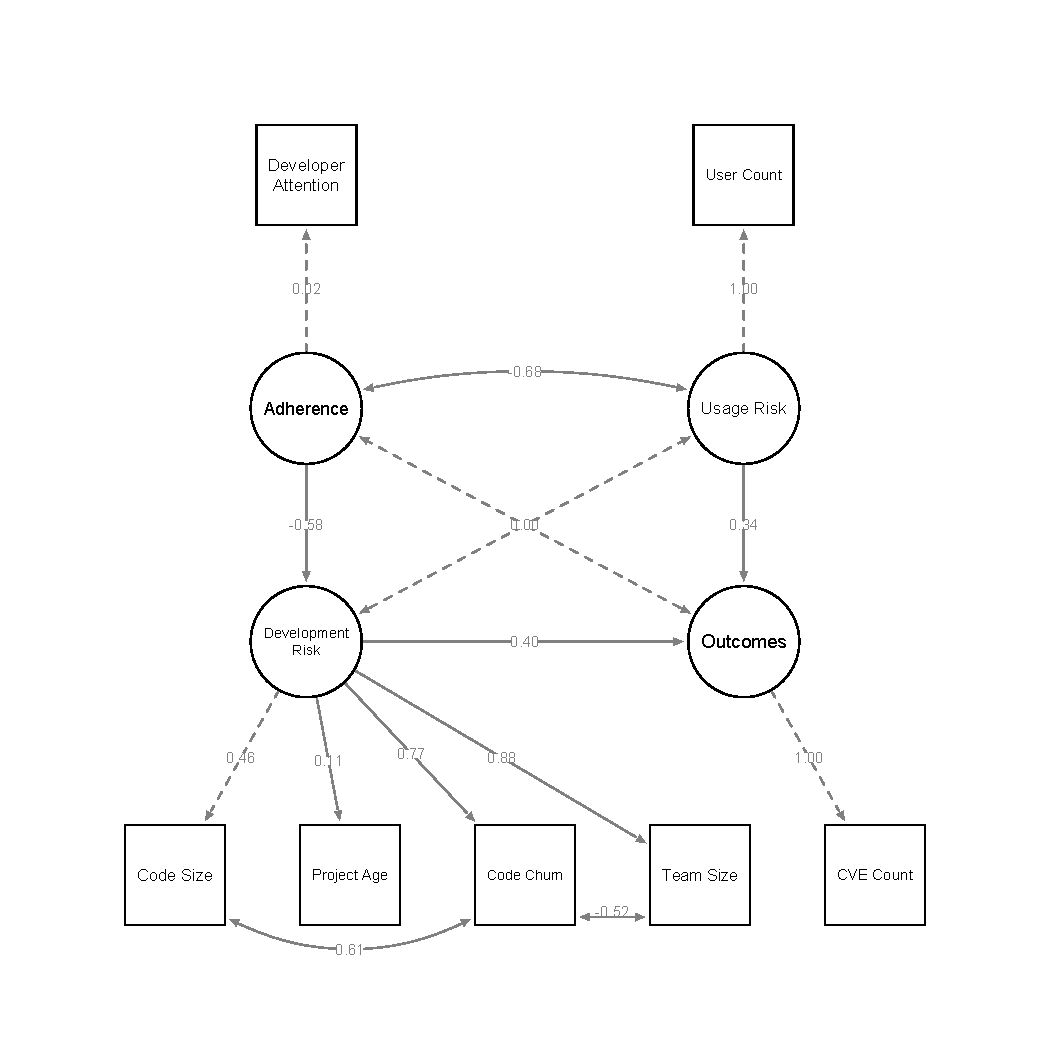
\includegraphics[width=1\textwidth]{Openhub_Respecified_SEM_Model.pdf}
	\caption{Respecified OpenHub-NVD Combine Model}
	\label{fig:openhub_model_respecified_estimates}
\end{figure*}

Interpreting the (standardized) parameter estimates in terms of our hypothesized construct relationships, we have the following:
\begin{itemize}
	\item  Usage Risk is positively associated (0.34) with Security Outcomes, as hypothesized. With an alpha of 0.07, Usage Risk is not significant at the .05 level, but is significant at the 0.10 level.
	\item Development Risk is positively associated (0.40) with Security Outcomes, as hypothesized. With an alpha of 0.07, Development Risk is not significant at the .05 level, but is significant at the 0.10 level.
	\item Practice Adherence is negatively associated ($-0.58$) with Development Risk, as hypothesized. With an alpha of 0.18, Usage Risk is not significant.
\end{itemize}	 

The residual variance values, shown in Table \ref{tab:results_openhub_residuals}, are lower than the .10 guideline established in Kline~\cite{kline2015principles}, with the exception of total\_code\_line's relationship with project\_age, and user\_count's relationship with project\_age. 

% stargazer(round(residuals(fitX)$cov,2),style="asr",digits=2)
% Table created by stargazer v.5.2 by Marek Hlavac, Harvard University. E-mail: hlavac at fas.harvard.edu
% Date and time: Tue, May 16, 2017 - 13:02:55
\begin{table}[!htbp] \centering 
  \caption{OpenHub-NVD Respecified Model Residuals} 
  \label{tab:results_openhub_residuals} 
\begin{tabular}{@{\extracolsep{0pt}}lrrrrrrr} 
\\[-1.8ex]\hline 
\hline \\[-1.8ex] 
 & $1.$ & $2.$ & $3.$ & $4.$ & $5.$ & $6.$ & $7.$ \\ 
\hline \\[-1.8ex] 
1. total\_code\_lines & $0$ & $0.11$ & $0$ & $0$ & $$-$0.05$ & $$-$0.01$ & $0.02$ \\ 
2. project\_age & $0.11$ & $0$ & $$-$0.03$ & $0.05$ & $0.04$ & $$-$0.05$ & $0.21$ \\ 
3. code\_churn\_12months & $0$ & $$-$0.03$ & $0$ & $0$ & $$-$0.01$ & $0$ & $0.01$ \\ 
4. twelve\_month\_contributor\_count & $0$ & $0.05$ & $0$ & $0$ & $$-$0.01$ & $0$ & $$-$0.01$ \\ 
5. CVECount & $$-$0.05$ & $0.04$ & $$-$0.01$ & $$-$0.01$ & $0$ & $0$ & $0$ \\ 
6. DevAttention & $$-$0.01$ & $$-$0.05$ & $0$ & $0$ & $0$ & $0$ & $0$ \\ 
7. user\_count & $0.02$ & $0.21$ & $0.01$ & $$-$0.01$ & $0$ & $0$ & $0$ \\
\hline \\[-1.8ex] 
\end{tabular} 
\end{table}
